\documentclass{beamer}
\usepackage{../../../resources/themes/algolymp-light}
\usepackage{booktabs}
\usetikzlibrary{matrix}

\title{Tablouri bidimensionale pătratice}
\subtitle{Delimitarea zonelor}
\author{Andrei Mihai Ciobanu}
\institute{Algolymp Summer School}
\date{}
\titlegraphic{
\includegraphics[width=3cm]{../../../resources/algolymp-logo.png}}
\setbeamertemplate{frame footer}{Algolymp Summer School}

% ================================================================
\begin{document}

\begin{frame}
  \titlepage
\end{frame}

\begin{frame}{Cuprins}
  \tableofcontents[hideallsubsections]
\end{frame}

% ================================================================
\section{Introducere}

\begin{frame}{Recapitulare — matricea pătratică}
  O matrice este \textbf{pătratică} când numărul de linii este egal cu numărul de coloane: $n = m$.

  \smallskip
  Folosim o singură variabilă $n$ pentru ambele dimensiuni.

  \smallskip
  \begin{center}
  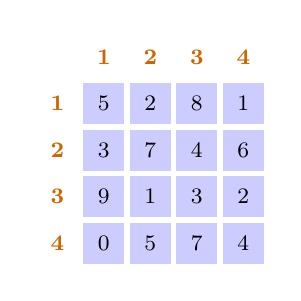
\begin{tikzpicture}
  \matrix[matrix of nodes,
          nodes in empty cells,
          ampersand replacement=\&,
          nodes={minimum size=0.52cm, text width=0.52cm, inner sep=0pt,
                 align=center, font=\footnotesize,
                 execute at begin node={\vphantom{0}}},
          row sep=2pt, column sep=2pt] {
    {} \& |[font=\footnotesize\bfseries, text=orange!80!black]| 1
       \& |[font=\footnotesize\bfseries, text=orange!80!black]| 2
       \& |[font=\footnotesize\bfseries, text=orange!80!black]| 3
       \& |[font=\footnotesize\bfseries, text=orange!80!black]| 4 \\
    |[font=\footnotesize\bfseries, text=orange!80!black]| 1
       \& |[fill=blue!20]| 5 \& |[fill=blue!20]| 2
       \& |[fill=blue!20]| 8 \& |[fill=blue!20]| 1 \\
    |[font=\footnotesize\bfseries, text=orange!80!black]| 2
       \& |[fill=blue!20]| 3 \& |[fill=blue!20]| 7
       \& |[fill=blue!20]| 4 \& |[fill=blue!20]| 6 \\
    |[font=\footnotesize\bfseries, text=orange!80!black]| 3
       \& |[fill=blue!20]| 9 \& |[fill=blue!20]| 1
       \& |[fill=blue!20]| 3 \& |[fill=blue!20]| 2 \\
    |[font=\footnotesize\bfseries, text=orange!80!black]| 4
       \& |[fill=blue!20]| 0 \& |[fill=blue!20]| 5
       \& |[fill=blue!20]| 7 \& |[fill=blue!20]| 4 \\
  };
  \end{tikzpicture}
  \end{center}

  \smallskip
  Exemplu: $n = 4$, deci 4 linii și 4 coloane. Elementul \texttt{a[2][3] = 4}.
\end{frame}

% ================================================================
\section{Diagonalele}

\begin{frame}{Diagonala principală}
  Diagonala principală unește colțul \textbf{stânga-sus} cu colțul \textbf{dreapta-jos}.

  \smallskip
  \begin{columns}[T]
    \column{0.48\textwidth}
    \begin{center}
    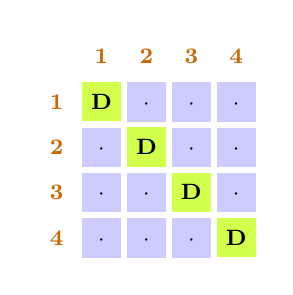
\begin{tikzpicture}
    \matrix[matrix of nodes,
            nodes in empty cells,
            ampersand replacement=\&,
            nodes={minimum size=0.50cm, text width=0.50cm, inner sep=0pt,
                   align=center, font=\footnotesize,
                   execute at begin node={\vphantom{0}}},
            row sep=2pt, column sep=2pt] {
      {} \& |[font=\footnotesize\bfseries, text=orange!80!black]| 1
         \& |[font=\footnotesize\bfseries, text=orange!80!black]| 2
         \& |[font=\footnotesize\bfseries, text=orange!80!black]| 3
         \& |[font=\footnotesize\bfseries, text=orange!80!black]| 4 \\
      |[font=\footnotesize\bfseries, text=orange!80!black]| 1
         \& |[fill=lime!70]| \textbf{D} \& |[fill=blue!20]| $\cdot$
         \& |[fill=blue!20]| $\cdot$    \& |[fill=blue!20]| $\cdot$ \\
      |[font=\footnotesize\bfseries, text=orange!80!black]| 2
         \& |[fill=blue!20]| $\cdot$    \& |[fill=lime!70]| \textbf{D}
         \& |[fill=blue!20]| $\cdot$    \& |[fill=blue!20]| $\cdot$ \\
      |[font=\footnotesize\bfseries, text=orange!80!black]| 3
         \& |[fill=blue!20]| $\cdot$    \& |[fill=blue!20]| $\cdot$
         \& |[fill=lime!70]| \textbf{D} \& |[fill=blue!20]| $\cdot$ \\
      |[font=\footnotesize\bfseries, text=orange!80!black]| 4
         \& |[fill=blue!20]| $\cdot$    \& |[fill=blue!20]| $\cdot$
         \& |[fill=blue!20]| $\cdot$    \& |[fill=lime!70]| \textbf{D} \\
    };
    \end{tikzpicture}
    \end{center}

    \column{0.52\textwidth}
    \begin{block}{Condiție}
      Un element \texttt{a[i][j]} este pe diagonala principală dacă:
      \[ i = j \]
    \end{block}

    \smallskip
    Exemple pentru $n = 4$:
    \begin{itemize}
      \item \texttt{a[1][1]}, \texttt{a[2][2]}, \texttt{a[3][3]}, \texttt{a[4][4]}
    \end{itemize}

    \smallskip
    Diagonala principală are \textbf{$n$ elemente}.
  \end{columns}
\end{frame}

\begin{frame}{Diagonala secundară}
  Diagonala secundară unește colțul \textbf{dreapta-sus} cu colțul \textbf{stânga-jos}.

  \smallskip
  \begin{columns}[T]
    \column{0.48\textwidth}
    \begin{center}
    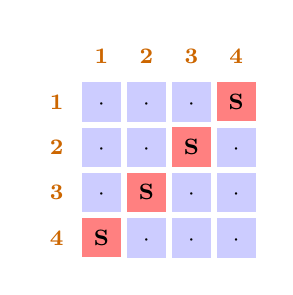
\begin{tikzpicture}
    \matrix[matrix of nodes,
            nodes in empty cells,
            ampersand replacement=\&,
            nodes={minimum size=0.50cm, text width=0.50cm, inner sep=0pt,
                   align=center, font=\footnotesize,
                   execute at begin node={\vphantom{0}}},
            row sep=2pt, column sep=2pt] {
      {} \& |[font=\footnotesize\bfseries, text=orange!80!black]| 1
         \& |[font=\footnotesize\bfseries, text=orange!80!black]| 2
         \& |[font=\footnotesize\bfseries, text=orange!80!black]| 3
         \& |[font=\footnotesize\bfseries, text=orange!80!black]| 4 \\
      |[font=\footnotesize\bfseries, text=orange!80!black]| 1
         \& |[fill=blue!20]| $\cdot$    \& |[fill=blue!20]| $\cdot$
         \& |[fill=blue!20]| $\cdot$    \& |[fill=red!50]| \textbf{S} \\
      |[font=\footnotesize\bfseries, text=orange!80!black]| 2
         \& |[fill=blue!20]| $\cdot$    \& |[fill=blue!20]| $\cdot$
         \& |[fill=red!50]| \textbf{S}  \& |[fill=blue!20]| $\cdot$ \\
      |[font=\footnotesize\bfseries, text=orange!80!black]| 3
         \& |[fill=blue!20]| $\cdot$    \& |[fill=red!50]| \textbf{S}
         \& |[fill=blue!20]| $\cdot$    \& |[fill=blue!20]| $\cdot$ \\
      |[font=\footnotesize\bfseries, text=orange!80!black]| 4
         \& |[fill=red!50]| \textbf{S}  \& |[fill=blue!20]| $\cdot$
         \& |[fill=blue!20]| $\cdot$    \& |[fill=blue!20]| $\cdot$ \\
    };
    \end{tikzpicture}
    \end{center}

    \column{0.52\textwidth}
    \begin{block}{Condiție}
      Un element \texttt{a[i][j]} este pe diagonala secundară dacă:
      \[ i + j = n + 1 \]
    \end{block}

    \smallskip
    Exemple ($n = 4$, deci $n + 1 = 5$):
    \begin{itemize}
      \item \texttt{a[1][4]}: $1 + 4 = 5$ \checkmark
      \item \texttt{a[2][3]}: $2 + 3 = 5$ \checkmark
      \item \texttt{a[3][2]}: $3 + 2 = 5$ \checkmark
      \item \texttt{a[4][1]}: $4 + 1 = 5$ \checkmark
    \end{itemize}
  \end{columns}
\end{frame}

\begin{frame}[fragile]{Parcurgerea diagonalelor}
  \begin{columns}[T]
    \column{0.5\textwidth}
    \textbf{Diagonala principală:}
    \begin{lstlisting}
for (int i = 1; i <= n; i++)
    cout << a[i][i] << ' ';
    \end{lstlisting}
    Condiție: \texttt{i == j}

    \column{0.5\textwidth}
    \textbf{Diagonala secundară:}
    \begin{lstlisting}
for (int i = 1; i <= n; i++)
    cout << a[i][n+1-i] << ' ';
    \end{lstlisting}
    Condiție: \texttt{i+j == n+1}
  \end{columns}

  \beginnote{Dacă $n$ este impar, centrul \texttt{a[(n+1)/2][(n+1)/2]} se află \textbf{pe ambele} diagonale simultan.}
\end{frame}

% ================================================================
\section{Zonele delimitate de diagonale}

\begin{frame}{Trei zone față de diagonala principală}
  \begin{columns}[T]
    \column{0.45\textwidth}
    \begin{center}
    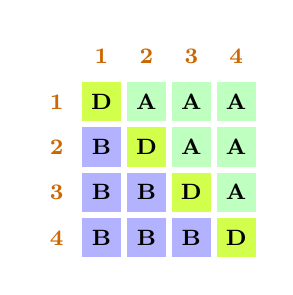
\begin{tikzpicture}
    \matrix[matrix of nodes,
            nodes in empty cells,
            ampersand replacement=\&,
            nodes={minimum size=0.50cm, text width=0.50cm, inner sep=0pt,
                   align=center, font=\footnotesize,
                   execute at begin node={\vphantom{0}}},
            row sep=2pt, column sep=2pt] {
      {} \& |[font=\footnotesize\bfseries, text=orange!80!black]| 1
         \& |[font=\footnotesize\bfseries, text=orange!80!black]| 2
         \& |[font=\footnotesize\bfseries, text=orange!80!black]| 3
         \& |[font=\footnotesize\bfseries, text=orange!80!black]| 4 \\
      |[font=\footnotesize\bfseries, text=orange!80!black]| 1
         \& |[fill=lime!70]| \textbf{D} \& |[fill=green!25]| \textbf{A}
         \& |[fill=green!25]| \textbf{A} \& |[fill=green!25]| \textbf{A} \\
      |[font=\footnotesize\bfseries, text=orange!80!black]| 2
         \& |[fill=blue!30]| \textbf{B} \& |[fill=lime!70]| \textbf{D}
         \& |[fill=green!25]| \textbf{A} \& |[fill=green!25]| \textbf{A} \\
      |[font=\footnotesize\bfseries, text=orange!80!black]| 3
         \& |[fill=blue!30]| \textbf{B} \& |[fill=blue!30]| \textbf{B}
         \& |[fill=lime!70]| \textbf{D} \& |[fill=green!25]| \textbf{A} \\
      |[font=\footnotesize\bfseries, text=orange!80!black]| 4
         \& |[fill=blue!30]| \textbf{B} \& |[fill=blue!30]| \textbf{B}
         \& |[fill=blue!30]| \textbf{B} \& |[fill=lime!70]| \textbf{D} \\
    };
    \end{tikzpicture}
    \end{center}

    \column{0.55\textwidth}
    \begin{itemize}
      \item \colorbox{lime!70}{\textbf{D}} \textbf{Pe diagonală:} $i = j$
      \item \colorbox{green!25}{\textbf{A}} \textbf{Deasupra:} $i < j$
      \item \colorbox{blue!30}{\textbf{B}} \textbf{Sub diagonală:} $i > j$
    \end{itemize}
    \begin{block}{Regulă simplă}
      Dacă linia e \textbf{mai mică} decât coloana $\rightarrow$ deasupra.\\
      Dacă linia e \textbf{mai mare} decât coloana $\rightarrow$ sub.
    \end{block}
  \end{columns}
\end{frame}

\begin{frame}[fragile]{Exemplu: suma pe zone față de diag. principală}
  \begin{lstlisting}
long long sD = 0; // suma de pe diagonala principala
long long sA = 0; // suma de deasupra
long long sB = 0; // suma de sub

for (int i = 1; i <= n; i++)
    for (int j = 1; j <= n; j++) {
        if (i == j) sD += a[i][j];
        if (i < j)  sA += a[i][j];
        if (i > j)  sB += a[i][j];
    }
  \end{lstlisting}

  \begin{itemize}
    \item Parcurgem toată matricea o singură dată
    \item Fiecare element se încadrează în \textbf{exact una} din cele trei zone
  \end{itemize}
\end{frame}

% ================================================================

\begin{frame}{Trei zone față de diagonala secundară}
  \begin{columns}[T]
    \column{0.45\textwidth}
    \begin{center}
    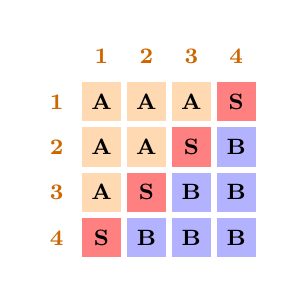
\begin{tikzpicture}
    \matrix[matrix of nodes,
            nodes in empty cells,
            ampersand replacement=\&,
            nodes={minimum size=0.50cm, text width=0.50cm, inner sep=0pt,
                   align=center, font=\footnotesize,
                   execute at begin node={\vphantom{0}}},
            row sep=2pt, column sep=2pt] {
      {} \& |[font=\footnotesize\bfseries, text=orange!80!black]| 1
         \& |[font=\footnotesize\bfseries, text=orange!80!black]| 2
         \& |[font=\footnotesize\bfseries, text=orange!80!black]| 3
         \& |[font=\footnotesize\bfseries, text=orange!80!black]| 4 \\
      |[font=\footnotesize\bfseries, text=orange!80!black]| 1
         \& |[fill=orange!30]| \textbf{A} \& |[fill=orange!30]| \textbf{A}
         \& |[fill=orange!30]| \textbf{A} \& |[fill=red!50]| \textbf{S} \\
      |[font=\footnotesize\bfseries, text=orange!80!black]| 2
         \& |[fill=orange!30]| \textbf{A} \& |[fill=orange!30]| \textbf{A}
         \& |[fill=red!50]| \textbf{S}    \& |[fill=blue!30]| \textbf{B} \\
      |[font=\footnotesize\bfseries, text=orange!80!black]| 3
         \& |[fill=orange!30]| \textbf{A} \& |[fill=red!50]| \textbf{S}
         \& |[fill=blue!30]| \textbf{B}   \& |[fill=blue!30]| \textbf{B} \\
      |[font=\footnotesize\bfseries, text=orange!80!black]| 4
         \& |[fill=red!50]| \textbf{S}    \& |[fill=blue!30]| \textbf{B}
         \& |[fill=blue!30]| \textbf{B}   \& |[fill=blue!30]| \textbf{B} \\
    };
    \end{tikzpicture}
    \end{center}

    \column{0.55\textwidth}
    Calculează $i + j$ și compară cu $n + 1$:

    \begin{itemize}
      \item \colorbox{red!50}{\textbf{S}} \textbf{Pe diagonală:} $i + j = n + 1$
      \item \colorbox{orange!30}{\textbf{A}} \textbf{Deasupra:} $i + j < n + 1$
      \item \colorbox{blue!30}{\textbf{B}} \textbf{Sub diagonală:} $i + j > n + 1$
    \end{itemize}
    \begin{block}{Exemplu ($n = 4$)}
      $n + 1 = 5$.
      Elementul \texttt{a[1][3]}: $1 + 3 = 4 < 5$ $\rightarrow$ deasupra.\\
      Elementul \texttt{a[3][4]}: $3 + 4 = 7 > 5$ $\rightarrow$ sub.
    \end{block}
  \end{columns}
\end{frame}

\begin{frame}[fragile]{Exemplu: suma pe zone față de diag. secundară}
  \begin{lstlisting}
long long sS = 0; // suma de pe diagonala secundara
long long sA = 0; // suma de deasupra
long long sB = 0; // suma de sub

for (int i = 1; i <= n; i++)
    for (int j = 1; j <= n; j++) {
        if (i + j == n + 1) sS += a[i][j];
        if (i + j < n + 1)  sA += a[i][j];
        if (i + j > n + 1)  sB += a[i][j];
    }
  \end{lstlisting}
\end{frame}

% ================================================================

\begin{frame}{Nord, Est, Sud, Vest}
  Cele două diagonale împart matricea în \textbf{4 zone} (pentru $n = 7$, $n+1 = 8$):

  \smallskip
  \begin{columns}[T]
    \column{0.54\textwidth}
    \begin{center}
    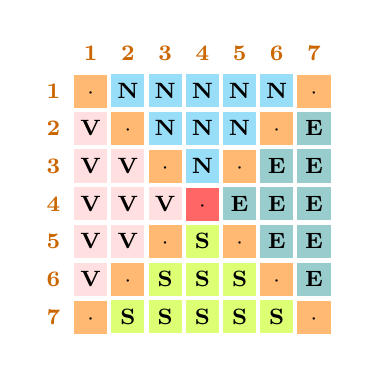
\begin{tikzpicture}
    \matrix[matrix of nodes,
            nodes in empty cells,
            ampersand replacement=\&,
            nodes={minimum size=0.42cm, text width=0.42cm, inner sep=0pt,
                   align=center, font=\footnotesize\bfseries,
                   execute at begin node={\vphantom{0}}},
            row sep=1.5pt, column sep=1.5pt] {
      % header
      {} \& |[font=\footnotesize\bfseries, text=orange!80!black]| 1
         \& |[font=\footnotesize\bfseries, text=orange!80!black]| 2
         \& |[font=\footnotesize\bfseries, text=orange!80!black]| 3
         \& |[font=\footnotesize\bfseries, text=orange!80!black]| 4
         \& |[font=\footnotesize\bfseries, text=orange!80!black]| 5
         \& |[font=\footnotesize\bfseries, text=orange!80!black]| 6
         \& |[font=\footnotesize\bfseries, text=orange!80!black]| 7 \\
      % row 1: DP N N N N N DS
      |[font=\footnotesize\bfseries, text=orange!80!black]| 1
         \& |[fill=orange!55]| $\cdot$
         \& |[fill=cyan!40]| N \& |[fill=cyan!40]| N
         \& |[fill=cyan!40]| N \& |[fill=cyan!40]| N
         \& |[fill=cyan!40]| N
         \& |[fill=orange!55]| $\cdot$ \\
      % row 2: V DP N N N DS E
      |[font=\footnotesize\bfseries, text=orange!80!black]| 2
         \& |[fill=pink!50]| V
         \& |[fill=orange!55]| $\cdot$
         \& |[fill=cyan!40]| N \& |[fill=cyan!40]| N
         \& |[fill=cyan!40]| N
         \& |[fill=orange!55]| $\cdot$
         \& |[fill=teal!40]| E \\
      % row 3: V V DP N DS E E
      |[font=\footnotesize\bfseries, text=orange!80!black]| 3
         \& |[fill=pink!50]| V \& |[fill=pink!50]| V
         \& |[fill=orange!55]| $\cdot$
         \& |[fill=cyan!40]| N
         \& |[fill=orange!55]| $\cdot$
         \& |[fill=teal!40]| E \& |[fill=teal!40]| E \\
      % row 4: V V V DP+DS E E E
      |[font=\footnotesize\bfseries, text=orange!80!black]| 4
         \& |[fill=pink!50]| V \& |[fill=pink!50]| V
         \& |[fill=pink!50]| V
         \& |[fill=red!60]| $\cdot$
         \& |[fill=teal!40]| E \& |[fill=teal!40]| E
         \& |[fill=teal!40]| E \\
      % row 5: V V DS S DP E E
      |[font=\footnotesize\bfseries, text=orange!80!black]| 5
         \& |[fill=pink!50]| V \& |[fill=pink!50]| V
         \& |[fill=orange!55]| $\cdot$
         \& |[fill=lime!55]| S
         \& |[fill=orange!55]| $\cdot$
         \& |[fill=teal!40]| E \& |[fill=teal!40]| E \\
      % row 6: V DS S S S DP E
      |[font=\footnotesize\bfseries, text=orange!80!black]| 6
         \& |[fill=pink!50]| V
         \& |[fill=orange!55]| $\cdot$
         \& |[fill=lime!55]| S \& |[fill=lime!55]| S
         \& |[fill=lime!55]| S
         \& |[fill=orange!55]| $\cdot$
         \& |[fill=teal!40]| E \\
      % row 7: DS S S S S S DP
      |[font=\footnotesize\bfseries, text=orange!80!black]| 7
         \& |[fill=orange!55]| $\cdot$
         \& |[fill=lime!55]| S \& |[fill=lime!55]| S
         \& |[fill=lime!55]| S \& |[fill=lime!55]| S
         \& |[fill=lime!55]| S
         \& |[fill=orange!55]| $\cdot$ \\
    };
    \end{tikzpicture}
    \end{center}

    \column{0.46\textwidth}
    \begin{tabular}{cl}
      \toprule
      Zonă & Condiție \\
      \midrule
      \colorbox{cyan!40}{\textbf{N}} Nord & $i < j$ și $i + j < n+1$ \\[2pt]
      \colorbox{teal!40}{\textbf{E}} Est  & $i < j$ și $i + j > n+1$ \\[2pt]
      \colorbox{lime!55}{\textbf{S}} Sud  & $i > j$ și $i + j > n+1$ \\[2pt]
      \colorbox{pink!50}{\textbf{V}} Vest & $i > j$ și $i + j < n+1$ \\
      \bottomrule
    \end{tabular}

    \smallskip
    \begin{block}{Observație}
      \colorbox{orange!55}{$\cdot$} diagonale \textemdash{} nu aparțin niciunei zone.\\
      \colorbox{red!60}{$\cdot$} centrul ($n$ impar) \textemdash{} pe ambele diagonale simultan.
    \end{block}
  \end{columns}
\end{frame}

\begin{frame}[fragile]{Exemplu: suma pe cele 4 zone}
  \begin{lstlisting}
long long sN = 0, sE = 0, sS = 0, sV = 0;

for (int i = 1; i <= n; i++)
    for (int j = 1; j <= n; j++) {
        if (i < j && i + j < n + 1) sN += a[i][j];
        if (i < j && i + j > n + 1) sE += a[i][j];
        if (i > j && i + j > n + 1) sS += a[i][j];
        if (i > j && i + j < n + 1) sV += a[i][j];
    }
  \end{lstlisting}

  \begin{itemize}
    \item Elementele de pe diagonale \textbf{nu} intră în nicio zonă
    \item Restul elementelor aparțin \textbf{exact uneia} din cele 4 zone
  \end{itemize}
\end{frame}

% ================================================================
\section{Recapitulare}


\begin{frame}{Probleme de antrenament}
  \begin{enumerate}
    \footnotesize\itemsep0pt
    \item \href{https://www.pbinfo.ro/probleme/313/diagonale}{\textbf{Diagonale}}
          \textcolor{gray}{(pbinfo \#313)}
    \item \href{https://code.algolymp.com/problems/4208}{\textbf{Four Zones of a Square Matrix}}
          \textcolor{gray}{(AlgoCode \#4208)}
    \item \href{https://www.pbinfo.ro/probleme/783/diagonale1}{\textbf{Diagonale1}}
          \textcolor{gray}{(pbinfo \#783)}
    \item \href{https://www.pbinfo.ro/probleme/4695/max-patrat}{\textbf{max\_patrat}}
          \textcolor{gray}{(pbinfo \#4695)}
    \item \href{https://www.pbinfo.ro/probleme/4578/dodel}{\textbf{Dodel}}
          \textcolor{gray}{(pbinfo \#4578)}
    \item \href{https://www.pbinfo.ro/probleme/4691/matrice19}{\textbf{Matrice19}}
          \textcolor{gray}{(pbinfo \#4691)}
    \item \href{https://www.pbinfo.ro/probleme/782/zona1}{\textbf{Zona1}}
          \textcolor{gray}{(pbinfo \#782)}
  \end{enumerate}
\end{frame}

\begin{frame}{Resurse}
  \begin{enumerate}
    \item \href{https://www.pbinfo.ro/articole/5626/tablouri-patratice}{\textbf{pbinfo.ro} \textemdash{} Tablouri pătratice}
    \item \href{https://www.pbinfo.ro/articole/5623/parcurgerea-tablourilor-bidimensionale}{\textbf{pbinfo.ro} \textemdash{} Parcurgerea tablourilor bidimensionale}
  \end{enumerate}
\end{frame}

\end{document}
